\section{Approach evaluation} \label{viability}

To verify the applicability of our detector and signature language, we tested the system by looking at several recent CVEs related to \ac{XSS}. We have three objectives: to verify that our signature language provides the necessary functionality to express an exploit and its patch, to test our detector against existing exploits, and to show that composing signatures takes a reasonable amount of time.

% does not incur a high time overhead when writing a signature.

\subsection{Methodology} \label{methodology}

We study recent CVEs related to WordPress
plugins. We focus on WordPress for two reasons:
%% While this may seem restrictive, there are several reasons
%% why we targeted WordPress plugins:
\begin{enumerate}
	\item WordPress powers 34.7\% of all websites according to a recent survey  \cite{w3stats} \cite{DBLP:journals/corr/abs-1801-01203}. The same study states that 30.3\% of the Alexa top 1000 sites use WordPress. Thus, we can be confident that our study results will hold true for the average user.
	\item WordPress plugins are popular among developers (there are currently more than 55,000 plugins \cite{wpplugins}). Due to its user popularity, WordPress is also heavily analyzed by security experts. A search for WordPress CVEs on the Mitre CVE database \cite{cvemitre} gives 2310 results. Plugins, specifically, are an important part of this issue, 52\% of the vulnerabilities reported by WPScan are caused by WordPress plugins \cite{wpscan}.
	%% \item WordPress plugin code is accessible, so we can easily analyze both the client-side HTML, as well as the server-side code that generated it, which is helpful when writing signatures.
	%% \item Using one framework, we can install many different plugins for the version we want, reproduce attacks, and investigate the conditions under which they happen, without having to install additional software.
\end{enumerate}

We used a CVE database, CVE Details~\cite{cvedetails} to
find the 100 most recent WordPress \ac{XSS} CVEs, as of
October 2018. %% We used a CVE database, CVE Details
%% \cite{cvedetails}, as opposed to other databases that include
%% vulnerabilities or exploits, mainly because of reliability. We have
%% been able to find hundreds of verified attacks on WordPress and its
%% plugins using a CVE database, which also usually contain information
%% on how to reproduce them. This provides the perfect platform to
%% analyze \ac{XSS} attacks and decide whether they can be countered by
%% our approach.
%
For each CVE, we set up a Docker container with a clean installation
of WordPress 5.2 and installed the vulnerable plugin's version. 
For CVEs that depended on a particular WordPress version, we
installed the appropriate version. Of the CVEs we looked at, only
one occurred in WordPress core. We believe it would be harder
to precisely sanitize injection points in WordPress core, as many of
the plugins have particular settings pages where the exploits occur,
and the HTML is more identifiable. WordPress core, on the other hand,
can be heavily altered by the use of themes and the user's own
changes. However, as evidenced by our investigation, the vast majority
of exploits occur in plugins.
 
Next, we reproduced the exploit in the CVE and we analyzed the
vulnerable page and wrote a signature to patch the exploit.

%%%%%%%%%%%%%%%%%%%%%%%%
\subsection{Results}
%%%%%%%%%%%%%%%%%%%%%%%%

\begin{table}[h!]
	\begin{center}
		\begin{tabular}{c c} 
			\hline
			\textbf{Plugin} & \textbf{Installations}\\ [1ex] 
			\hline
			WooCommerce  & 5+ million  \\  
			Duplicator & 1+ million \\  
			Loginizer & 900,000+ \\  
			WP Statistics & 500,000+ \\  
			Caldera Forms & 200,000+ \\   
			\hline
		\end{tabular}
		\caption{Most popular studied WordPress plugins}
		\label{table:1}
	\end{center}
\end{table}

Of the initial 100 CVEs, we were able to analyze 76 across 44 affected
pages. We dropped 24 CVEs due to reproducibility issues: some of the
descriptions did not include a PoC, making it difficult for us to
reproduce; or, the plugin code was no longer available. In some cases,
it had been removed from the WordPress repository due to "security
issues", which emphasizes the importance of being able to defend
against these attacks. %% This is not to say, however, that our detector
%% would not work for such a CVE, as the author would have a better idea
%% of how the exploit manifests itself, and would be in a better position
%% to write a signature.

The resulting plugins we studied averaged 489,927
installations: \autoref{table:1} shows the number of installations for
the 5 most popular plugins we studied. For the vulnerabilities, 27
(35.5\%) could be exploited by an unauthenticated user; 56 (73.7\%)
targeted a high-privilege user as the victim, 7 (9.2\%) had a
low-privilege user as the victim, the rest affected users of all
types.

Many of the studied CVEs included attacks for which there are known
and widely deployed defenses. For example, many were cases of
Reflected \ac{XSS}, where the URL revealed the existence of an attack,
e.g.,: \url{http://<target>&page-uri=<script>alert("\ac{XSS}")</script>}
While Chrome's built-in \ac{XSS} auditor blocked this request, Firefox
did not, and so we still wrote signatures for such attacks\footnote{In
practice, we found several cases where even XSS auditor did not block
a reflected XSS.}.

We wrote 59 WordPress signatures in total, which got rid of the PoC
exploit when sanitized with one of our three methods. Note that while
a PoC is often the most simple form of an attack, our sanitization
methods, and in particular DOMPurify, can get rid of complex
injections as well. We were able to include several CVEs in some PoCs
because they occurred in the same page and affected the same
plugin. Overall, these signatures represent 71 (93.4\%) signed
CVEs. The 5 we were not able to sign were due to lack of identifiers
in the HTML, which would result in potentially large chunks of the
document being replaced\footnote{In these cases, the signature developer
can weigh the trade-offs and decide whether the added cost is worth
it.}

After manual testing, the majority of the 71 signatures maintained the
same layout and core functionality of the webpage. However, 12
signatures caused some elements to be rearranged, modifying the page's
visual aspect. One caused a small part of the page to become unusable,
due to the sanitization method (a table showing user information
was now rendered as blank). Most of the responsibility of maintaining
functionality is left to the signature developer. We found that being precise
is key to retaining functionality. Furthermore, even if the layout of the page is
affected, we believe that applying the signature is preferable
to allowing an exploit. And, unlike the complete blocking approach commonly used by malware
detection software, our approach allows the user to access the page.

While our goal is to retain as much information of the page as
possible after sanitization, we believe that even if a part of the
page becomes unusable, this does not impact the user's experience as
much, since many of the exploits occur in small sections of the
HTML. A usability study is out of scope for this paper and we leave it
to future work.

%%  (see , but we provide some insight into false positives and false
%% negatives in 
%, which is related to this issue.

\subsection{Generalizability beyond WordPress}
\label{generalizability}

To test the generalizability of our approach to other frameworks, we
analyzed 5 additional CVEs, 2 related to Joomla!, 2 for LimeSurvey,
and 1 for Bolt CMS.  We chose Joomla! because it is another
popular \ac{CMS}. Unfortunately, we only found 2 CVEs
that we were able to reproduce, as the software for its extensions is
often not available. For fairness, we looked for the most recent CVEs
we could reproduce listed in the Exploit Database~\cite{exploitdb}, since
these have recorded \acp{PoC}. We carried out the same
procedure as with the WordPress CVEs, and were able to patch all of
the 5 exploits. This brought our CVE coverage rate up to 93.8\%.

\subsection{Signature writing times} \label{signature_times}

\autoref{fig:signature_times} plots a histogram of the times it took
one of the authors to compose each of the signatures. Each time
measurement includes the time it took to check the HTML injection
points, write the signature and to debug it. We do not include the
time taken to discover and carry out an exploit, as this is part of
the CVE writing process. The median time is 3.89 minutes, and the
standard deviation is 4.18 minutes. 72\% of signatures were written in
under 5 minutes. We believe this to be a reasonable amount of time
considering the security granted by our extension.

The signature which took the longest time to write (25 minutes)
corresponds to an exploit with 12 HTML injection points. Additionally,
testing this signature proved difficult, as some of
the injections were a result of a script inserting elements in the DOM
after the page had loaded. This caused the initial HTML to look
innocuous, but with exploits still occurring after sanitization. As
this script was part of the initial request, we eventually got to the
root of the problem. We believe a more experienced exploit analyst
might be able to detect this kind of behaviour more
easily. %% Furthermore, having so many injection points in the HTML is
%% cause for great complexity, and the writer can decide to block the
%% page entirely, which would bring down the time taken.

The signature which took the second longest time to write (18 minutes)
corresponds to an exploit with 7 injection points; each of
these belongs to a part of the HTML with generic element
identifiers. Our language provides a means to overcome this, by allowing
the developer to specify the element's "position": for example, if there are
three <h3 class="title"> elements, in the HTML, and only one of them
is an injection starting point, the writer can specify that the third
one needs to be sanitized. The same can be done for the ending points. As
there were 7 of such points, debugging took longer than for
other signatures.
%% Again, this is a complex case, and can be
%% more prone to user error than other signatures, the writer might
%% instead decide to block the page entirely.

%% Our dataset contained signatures which cover several CVEs, as
%% sometimes a single page is associated with multiple CVEs. We had 6
%% such pages. which had a median write time of 6.54 minutes. This means
%% that the time per CVE is lower than the overall median of
%% 3.89.
Another source of longer timings are complicated 
listener type signatures, like the ones for exploits caused by an
XHR. We had 4 such signatures and composed these with a median time of 9.86 minutes.
%% these had a median write time of 9.86.
As only a small number of these were present, we expect the time
taken to compose a typical signature to be lower than the overall median in this experiment.

\begin{figure}[h]
	\begin{center}
	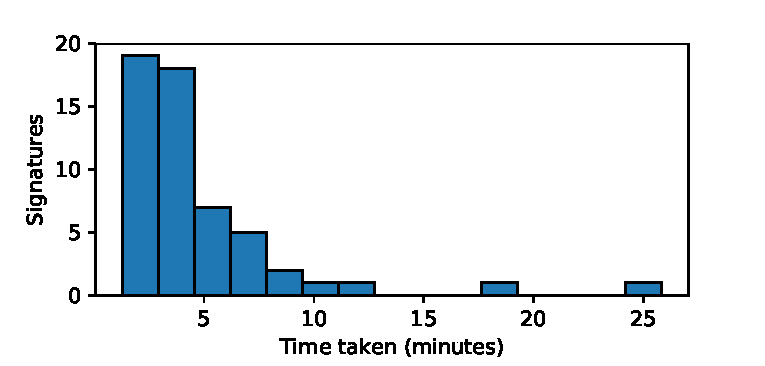
\includegraphics[width=\linewidth]{results/signature_times_small.pdf}
	\caption{Histogram of time taken to write signatures.}
	\label{fig:signature_times}
	\end{center}
\end{figure}


